% Multijet balance: data/MC x_j study (October 2026)
\documentclass[aspectratio=169,10pt]{beamer}
\usepackage[T1]{fontenc}
\usepackage[utf8]{inputenc}
\usepackage{booktabs}
\usepackage{graphicx}
\usepackage{xcolor}
\usepackage{amsmath}

\definecolor{navy}{HTML}{1D2733}
\definecolor{accent}{HTML}{2E6DA4}
\definecolor{good}{HTML}{3E7D5C}
\definecolor{bad}{HTML}{B23A38}
\setbeamercolor{frametitle}{fg=navy}
\setbeamercolor{structure}{fg=accent}
\setbeamercolor{title}{fg=navy}
\setbeamertemplate{navigation symbols}{}
\setbeamertemplate{itemize items}[circle]
\setbeamerfont{frametitle}{size=\Large,series=\bfseries}
\setbeamertemplate{footline}{\hfill\insertframenumber\,/\,\inserttotalframenumber\hspace{1em}\vspace{0.6em}}

\newcommand{\xj}{x_{j}}
\newcommand{\good}[1]{\textcolor{good}{#1}}
\newcommand{\bad}[1]{\textcolor{bad}{#1}}

\title{Multijet balance: finding the data/MC $\langle \xj \rangle$ bias}
\subtitle{Skim, sample stitching and JER smearing of the recoil jets}
\author{Samuel F.\ Liechty}
\date{October 6, 2026}

\begin{document}

\begin{frame}
  \titlepage
\end{frame}

% ------------------------------------------------------------------
\begin{frame}{The observable and the problem}
  \begin{itemize}
    \item Multijet balance $\xj = p_{T,\mathrm{lead}} / |\vec p_{T,2} + \vec p_{T,3}|$, in bins of leading-jet $p_T$, seven jet radii.
    \item Selection: leading $\geq 20$ GeV, jets 2 and 3 in $[7, 30)$ GeV, $|\eta| < 1.1 - R$, $\Delta\phi_{12} > 3\pi/4$, $\Delta\phi_{13} > \pi/2$.
    \item MC jets get an extra JER smearing, so that MC resolution matches data.
    \item With the original trees, data/MC of $\langle \xj \rangle$ was far from 1 (R = 0.4):
  \end{itemize}
  \vspace{0.5em}
  \centering
  \begin{tabular}{lccccc}
    \toprule
    leading $p_T$ (GeV) & 20--25 & 25--30 & 30--35 & 35--40 & 40--50 \\
    \midrule
    data/MC & \bad{1.077} & \bad{1.067} & \bad{1.063} & \bad{1.037} & \bad{1.034} \\
    \bottomrule
  \end{tabular}
  \vspace{0.8em}
  \begin{itemize}
    \item We expect this ratio to be within about 1\% of unity.
    \item The trigger requirement and a data JES of 0.93 were both tried and did not fix it.
  \end{itemize}
\end{frame}

% ------------------------------------------------------------------
\begin{frame}{Finding 1: the skim cut MC on a different $p_T$ than the analysis}
  \begin{columns}[T]
    \begin{column}{0.52\textwidth}
      \begin{itemize}
        \item The treemaker skimmed events on the unsmeared calibrated $p_T$ (leading $\geq 20$, jets 2 and 3 $\geq 7$ GeV).
        \item It also kept only the top three jets by calibrated $p_T$.
        \item The analysis cuts MC on the smeared $p_T$.
        \item Events that pass only after smearing were never written.
        \item These come mostly from the lower $\hat p_T$ samples and have high $\xj$.
        \item Cross sections and stitching thresholds were checked and are correct.
      \end{itemize}
    \end{column}
    \begin{column}{0.46\textwidth}
      \small
      \textbf{Fix in DijetTreeMaker:}
      \begin{itemize}
        \item MC: keep the event if any of the seven $p_T$ flavors passes (calib + six JER smears).
        \item Keep the union of each flavor's top three jets.
        \item Store jets if any flavor $\geq 5$ GeV.
        \item Data: skim thresholds $\times\,0.9$, for in-situ JES scans down to $p_a = 0.9$.
      \end{itemize}
    \end{column}
  \end{columns}
\end{frame}

% ------------------------------------------------------------------
\begin{frame}{The new skim recovers 3--4$\times$ more selected MC events}
  \begin{columns}[T]
    \begin{column}{0.56\textwidth}
      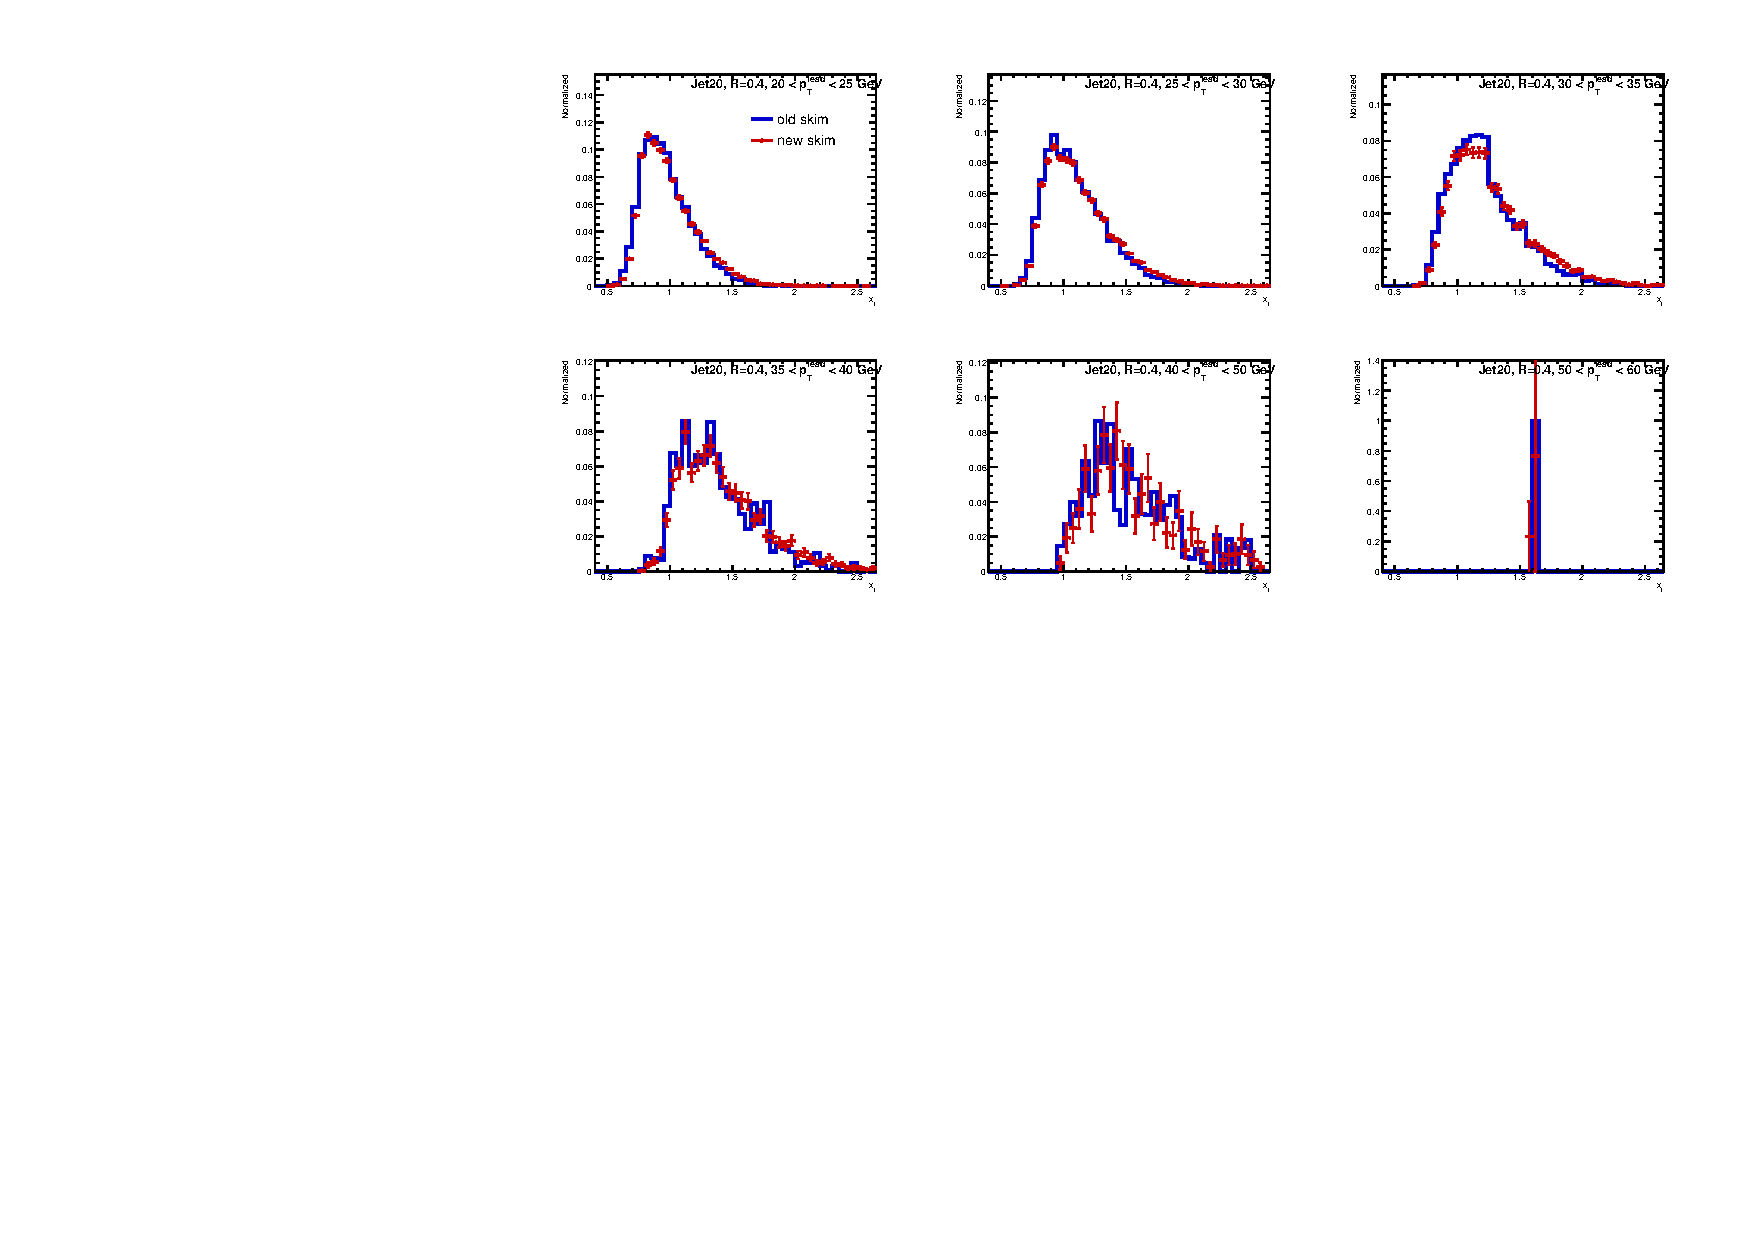
\includegraphics[width=\linewidth]{figs/skim_old_vs_new_jet20.pdf}
    \end{column}
    \begin{column}{0.42\textwidth}
      \small
      Jet20 sample, R = 0.4, same analysis code:
      \vspace{0.3em}

      \begin{tabular}{lcc}
        \toprule
        $p_T$ bin & events & $\langle\xj\rangle$ \\
        \midrule
        20--25 & $\times 4.2$ & 0.975 $\to$ 1.001 \\
        25--30 & $\times 3.6$ & 1.097 $\to$ 1.130 \\
        30--35 & $\times 3.3$ & 1.219 $\to$ 1.267 \\
        35--40 & $\times 3.1$ & 1.376 $\to$ 1.421 \\
        \bottomrule
      \end{tabular}
      \vspace{0.5em}
      \begin{itemize}
        \item About two thirds of the selected MC events were missing.
        \item The recovered events sit in the high-$\xj$ tail.
      \end{itemize}
    \end{column}
  \end{columns}
\end{frame}

% ------------------------------------------------------------------
\begin{frame}{Finding 2: Jet5 adds noise, so stitch from Jet12}
  \begin{columns}[T]
    \begin{column}{0.58\textwidth}
      \includegraphics[width=\linewidth,page=3]{figs/samples_with_jet5.pdf}
    \end{column}
    \begin{column}{0.40\textwidth}
      \small
      \begin{itemize}
        \item At fixed leading $p_T$, lower $\hat p_T$ samples have higher $\xj$.
        \item The MC mean is therefore sensitive to the sample mix.
        \item Jet5 carries 9.6\% of the 20--25 GeV weight from 9 events.
        \item In 25--30 GeV one Jet5 event carries 6.1\%.
        \item Jet8 has no MDC2 thresholds to stitch with Jet5.
        \item Jet5 and Jet8 are removed, and Jet12 starts at truth $p_T = 0$.
      \end{itemize}
    \end{column}
  \end{columns}
\end{frame}

% ------------------------------------------------------------------
\begin{frame}{After the new skim: a 2--3\% excess remains at low $p_T$}
  \begin{columns}[T]
    \begin{column}{0.44\textwidth}
      \includegraphics[width=\linewidth,page=7]{figs/means_jet12from0.pdf}
    \end{column}
    \begin{column}{0.54\textwidth}
      \small
      New MC trees, Jet12/20/30, R = 0.4, reco-anchored smearing:
      \vspace{0.3em}

      \begin{tabular}{lccccc}
        \toprule
        & 20--25 & 25--30 & 30--35 & 35--40 & 40--50 \\
        \midrule
        data/MC & 1.034 & 1.023 & 1.021 & 1.000 & 1.006 \\
        \bottomrule
      \end{tabular}
      \vspace{0.6em}

      Data vs weighted MC, 20--25 GeV bin:
      \vspace{0.3em}

      \begin{tabular}{lc}
        \toprule
        quantity & data/MC \\
        \midrule
        $\langle p_{T,\mathrm{lead}} \rangle$ & 1.000 \\
        $\langle p_{T,2} \rangle$ & \bad{0.935} \\
        $\langle p_{T,3} \rangle$ & \bad{0.956} \\
        \bottomrule
      \end{tabular}
      \vspace{0.4em}
      \begin{itemize}
        \item The reweighting closes; the MC recoil jets are too hard.
      \end{itemize}
    \end{column}
  \end{columns}
\end{frame}

% ------------------------------------------------------------------
\begin{frame}{Finding 3: the extra smearing is very wide for soft jets}
  \begin{columns}[T]
    \begin{column}{0.50\textwidth}
      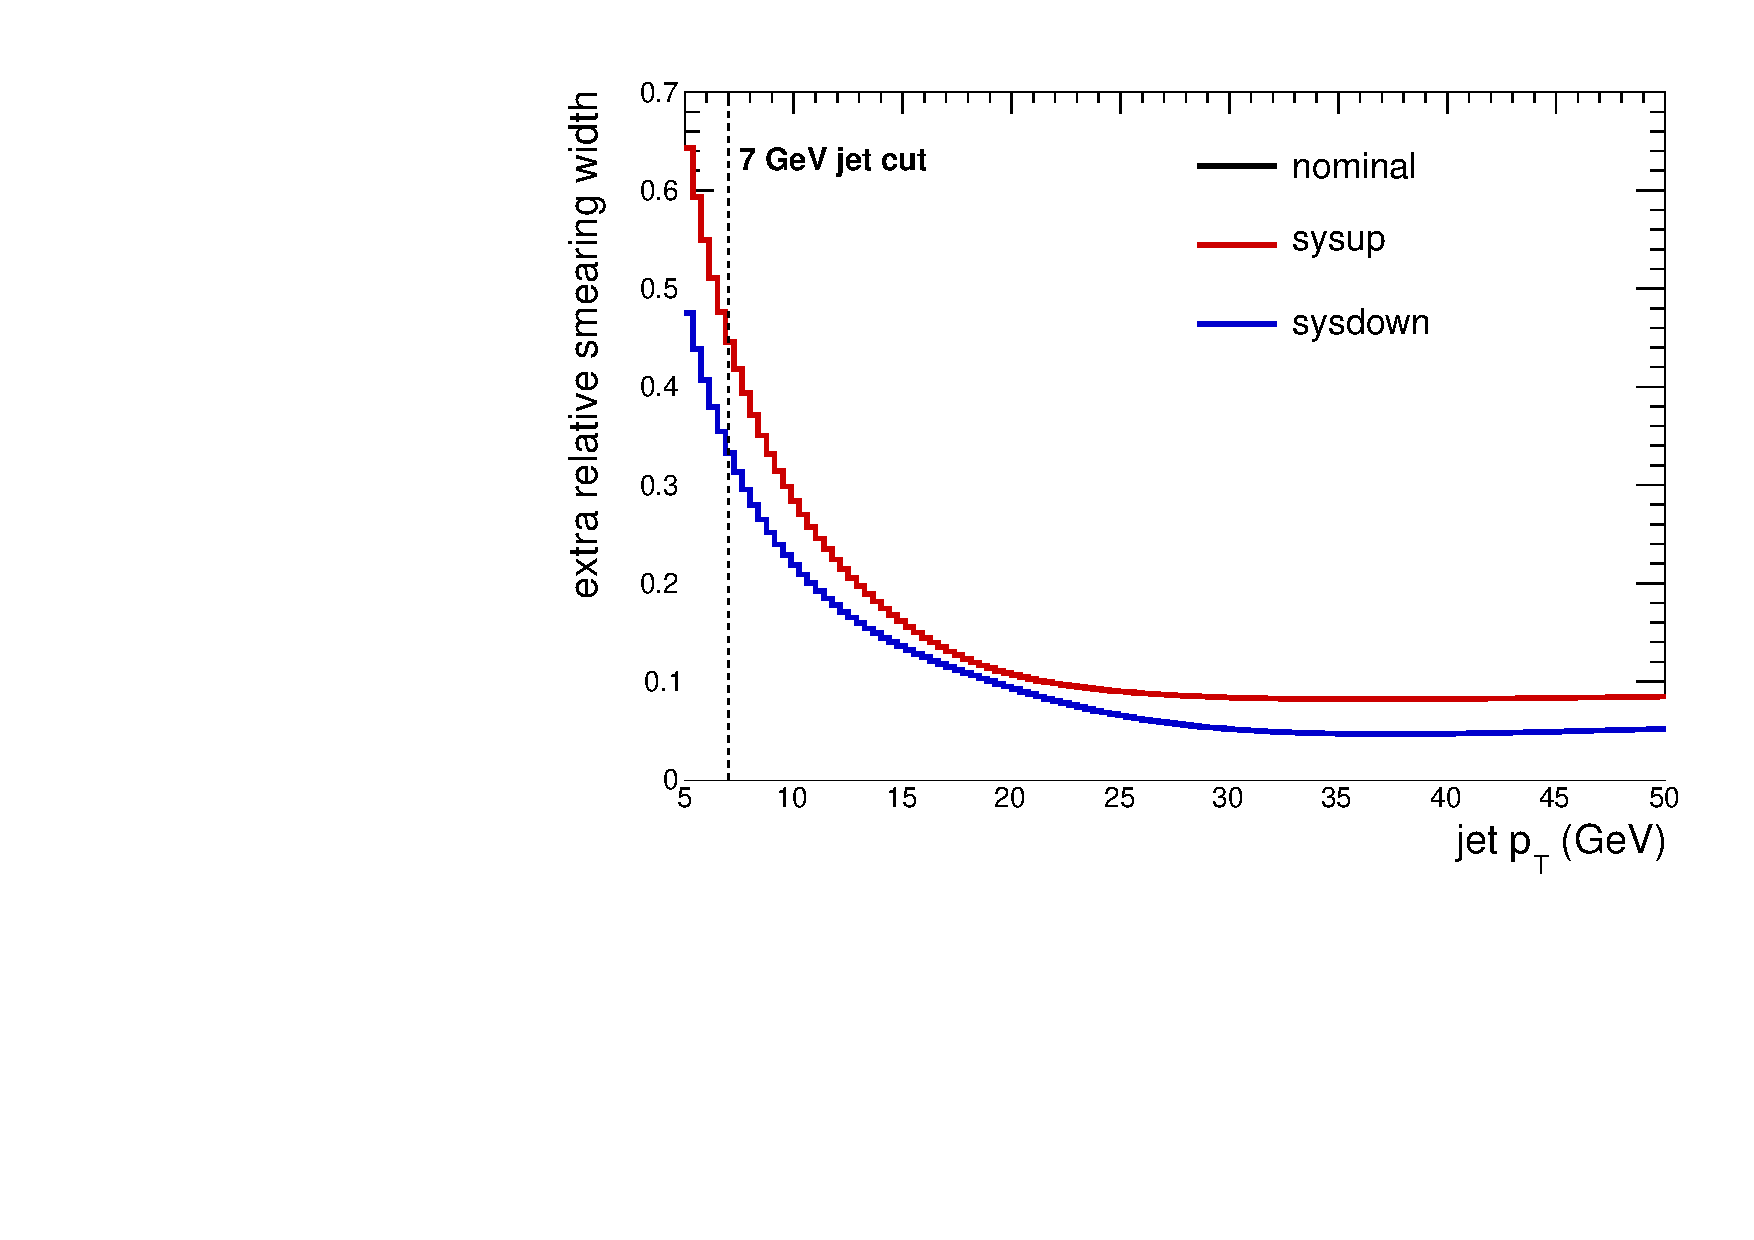
\includegraphics[width=\linewidth]{figs/jer_template_widths.pdf}
    \end{column}
    \begin{column}{0.48\textwidth}
      \small
      \begin{itemize}
        \item Template \texttt{h\_jer\_smear\_r04\_pileup\_EMfracJES}, used for every radius.
        \item Extra width: 39\% at 7 GeV, 25\% at 10 GeV, 10\% at 20 GeV.
        \item It is added on top of the MC's own resolution.
        \item Soft jets on a steep spectrum are pushed over the 7 GeV cut.
      \end{itemize}
      \vspace{0.3em}
      Test with no extra MC smearing (R = 0.4):
      \vspace{0.3em}

      \begin{tabular}{lccccc}
        \toprule
        & 20--25 & 25--30 & 30--35 & 35--40 \\
        \midrule
        smeared & 1.034 & 1.023 & 1.021 & 1.000 \\
        no smear & 0.991 & 0.997 & 1.000 & 0.991 \\
        \bottomrule
      \end{tabular}
    \end{column}
  \end{columns}
\end{frame}

% ------------------------------------------------------------------
\begin{frame}{The third jet usually has no truth jet above 7 GeV}
  \small
  Jet20, events passing the analysis 3-jet selection (smeared jets):
  fraction with $\leq 2$ truth jets.
  \vspace{0.5em}

  \centering
  \begin{tabular}{lccc}
    \toprule
    R & all stored truth jets ($\geq 3$ GeV) & truth $\geq 7$ GeV & truth $\geq 7$ GeV in acceptance \\
    \midrule
    0.2 & 13.5\% & 80.1\% & 82.5\% \\
    0.3 & 16.3\% & 76.4\% & 81.7\% \\
    0.4 & 16.6\% & 71.0\% & 81.4\% \\
    0.5 & 16.2\% & 66.3\% & 83.4\% \\
    0.6 & 17.5\% & 65.8\% & 87.6\% \\
    \bottomrule
  \end{tabular}
  \vspace{0.8em}
  \begin{itemize}
    \item In most selected MC events, jet 3 is a soft jet fluctuated over 7 GeV.
    \item About 1 in 6 has no third truth jet at all, so it is a fake or a split jet.
    \item This is why the result depends so strongly on the low-$p_T$ smearing width.
  \end{itemize}
\end{frame}

% ------------------------------------------------------------------
\begin{frame}{Event displays: the events we are correcting (1/3)}
  \begin{columns}[T]
    \begin{column}{0.29\textwidth}
      \centering
      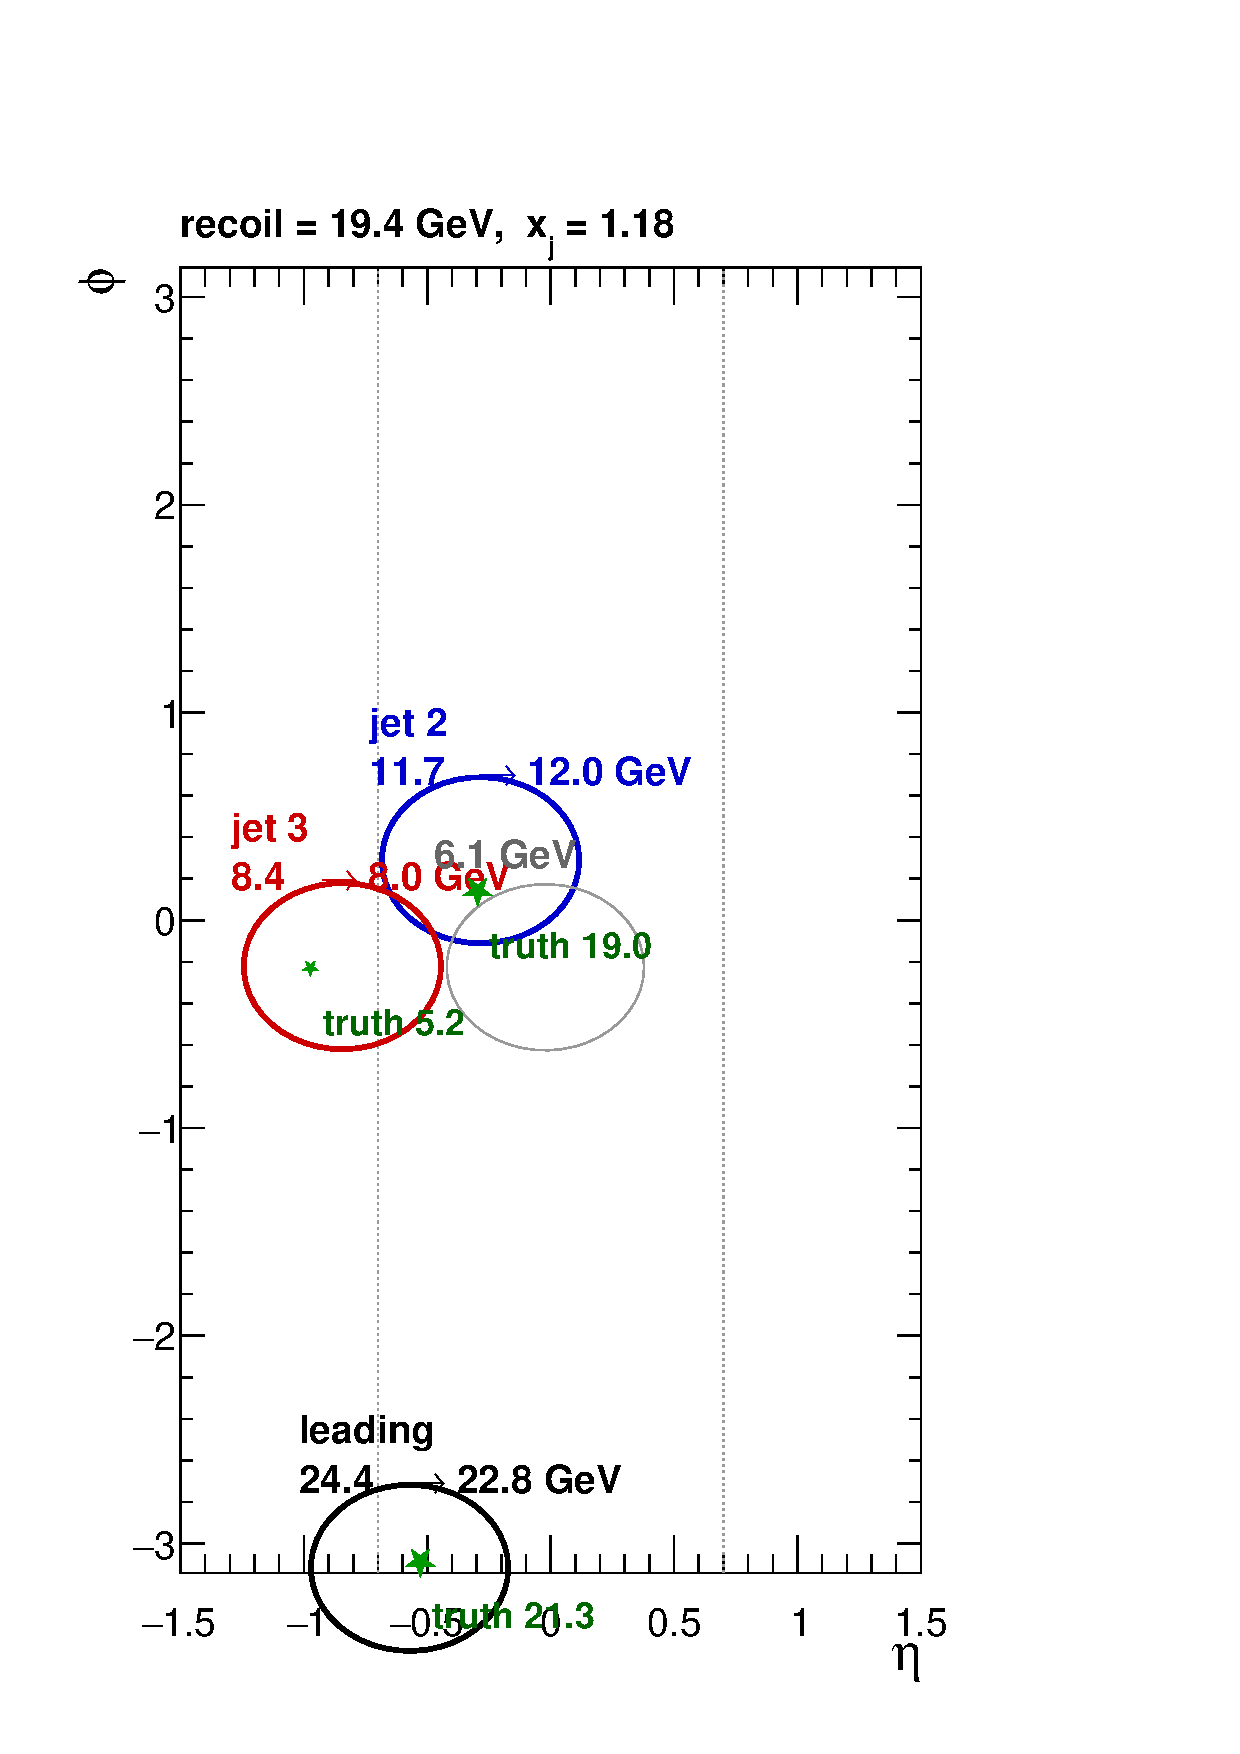
\includegraphics[height=0.83\textheight]{figs/event_display_0.pdf}
    \end{column}
    \begin{column}{0.29\textwidth}
      \centering
      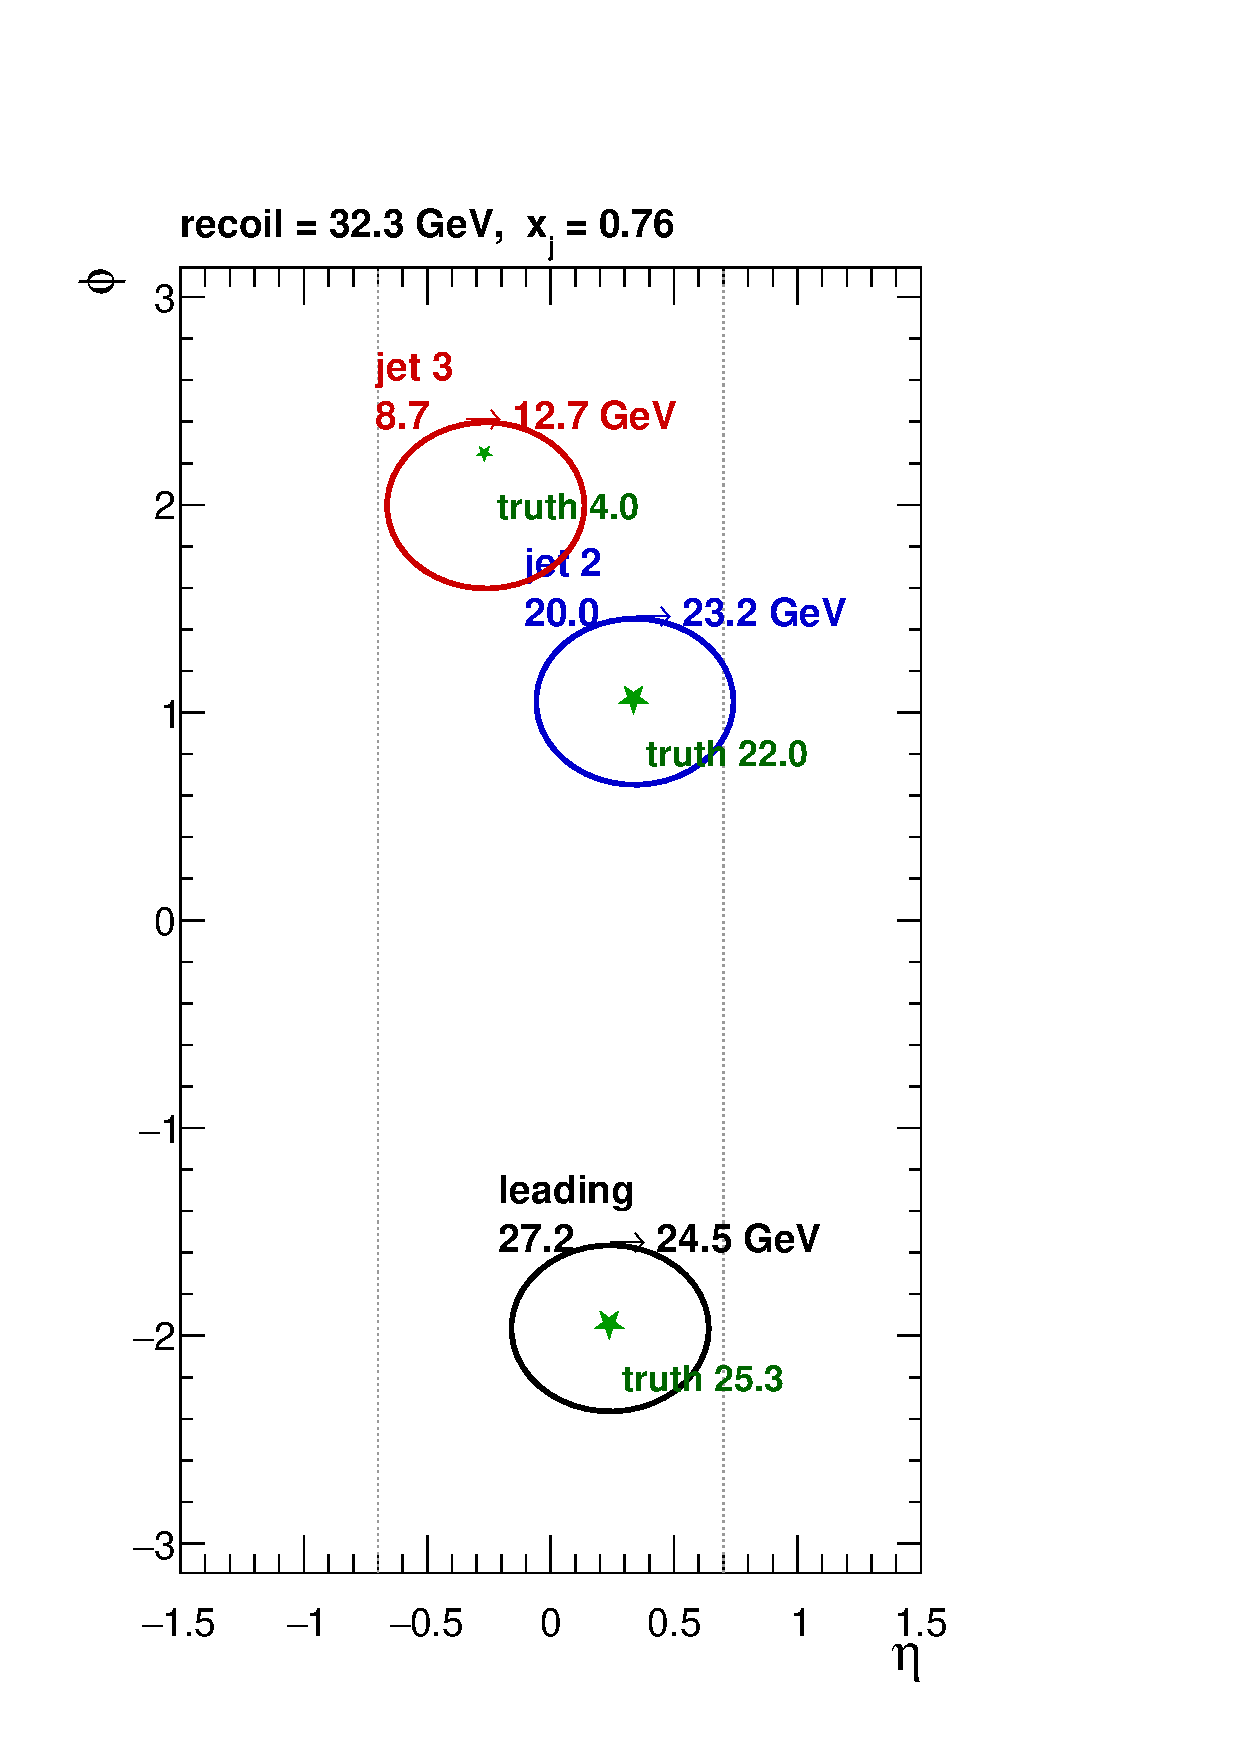
\includegraphics[height=0.83\textheight]{figs/event_display_2.pdf}
    \end{column}
    \begin{column}{0.38\textwidth}
      \small
      Pythia8 Jet20, R = 0.4: selected events with three reco jets but only two truth jets $\geq 7$ GeV.
      \vspace{0.4em}

      Reco jets show calibrated $\to$ smeared $p_T$; green stars are truth jets; dotted lines mark the acceptance.
      \vspace{0.4em}
      \begin{itemize}
        \item Left: jet 3 (8.4 GeV) sits on a 5.2 GeV truth jet.
        \item Right: jet 3 is smeared from 8.7 to 12.7 GeV on a 4.0 GeV truth jet.
      \end{itemize}
    \end{column}
  \end{columns}
\end{frame}

\begin{frame}{Event displays: the events we are correcting (2/3)}
  \begin{columns}[T]
    \begin{column}{0.29\textwidth}
      \centering
      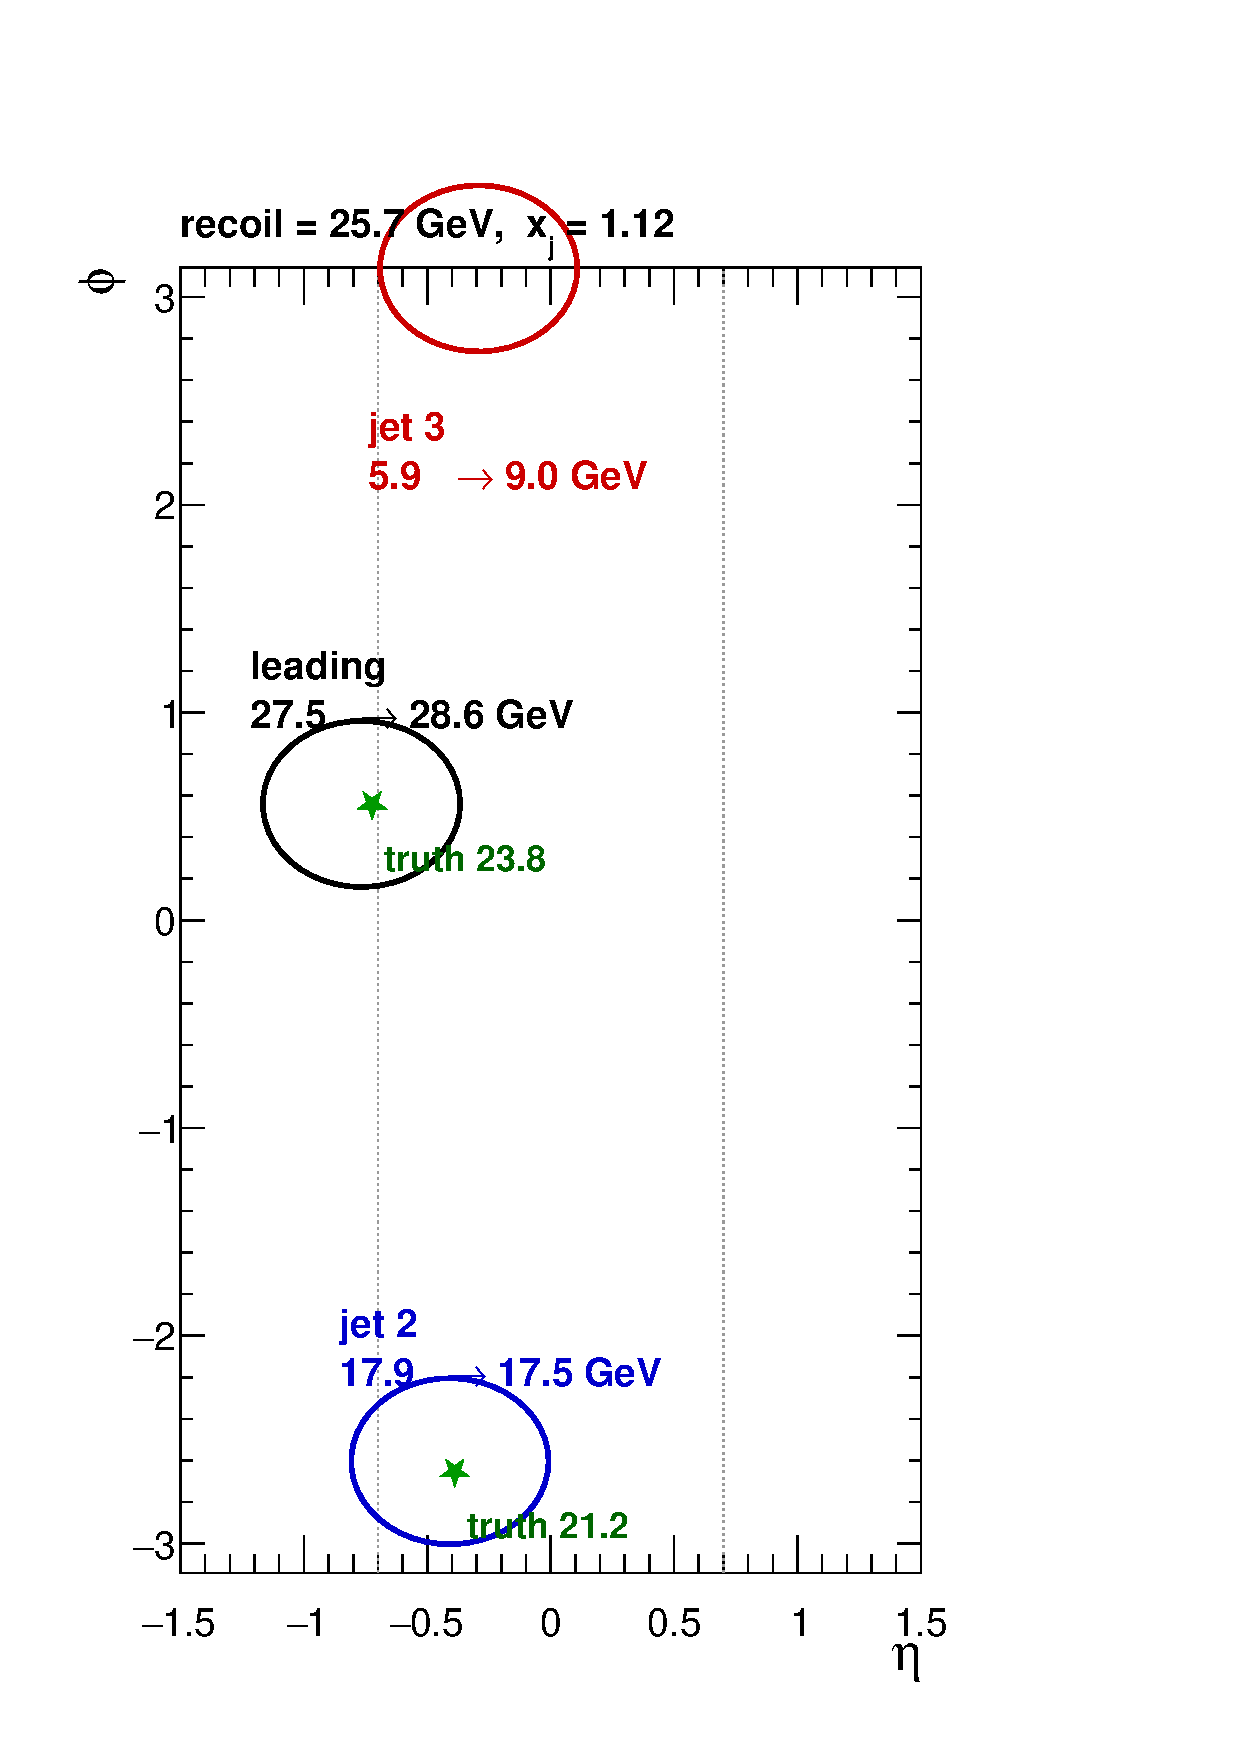
\includegraphics[height=0.83\textheight]{figs/event_display_4.pdf}
    \end{column}
    \begin{column}{0.29\textwidth}
      \centering
      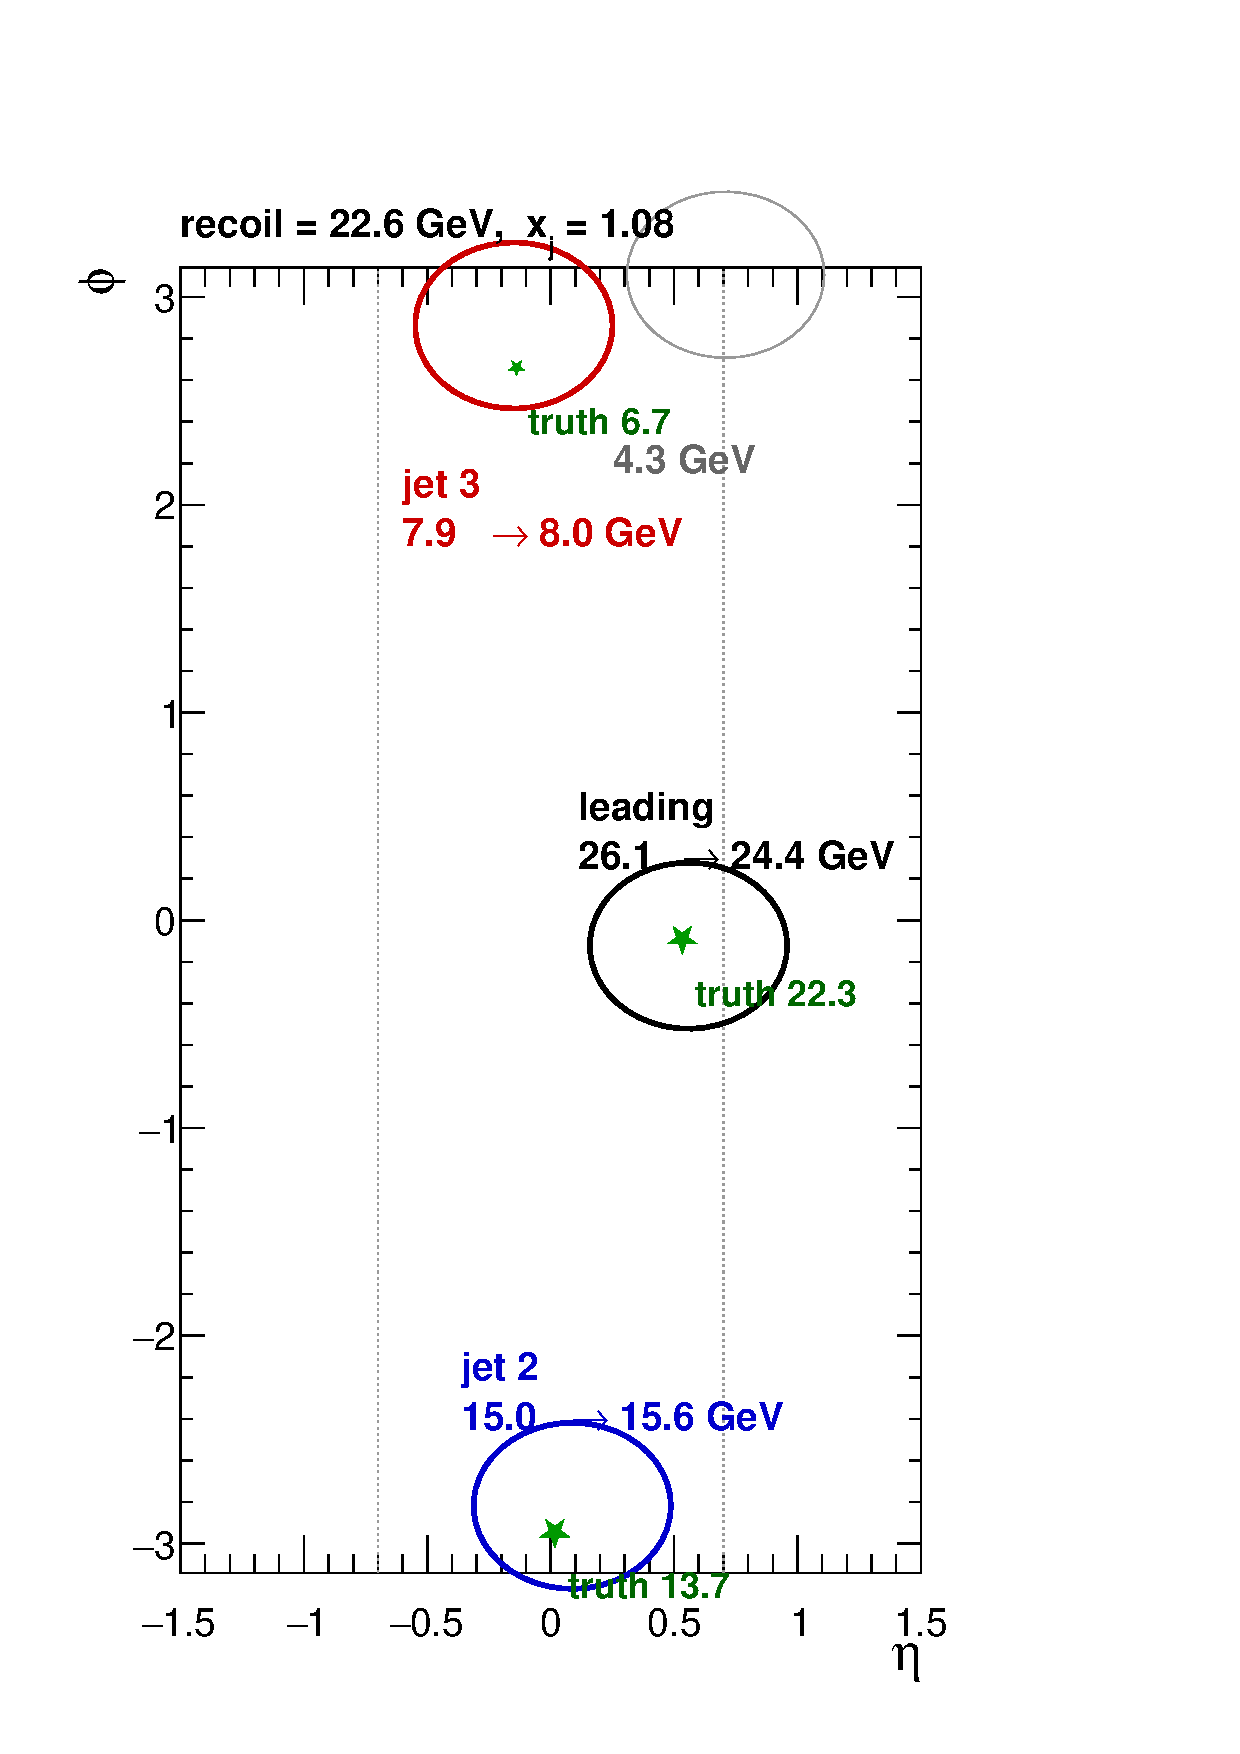
\includegraphics[height=0.83\textheight]{figs/event_display_1.pdf}
    \end{column}
    \begin{column}{0.38\textwidth}
      \small
      Pythia8 Jet20, R = 0.4: selected events with three reco jets but only two truth jets $\geq 7$ GeV.
      \vspace{0.4em}

      Reco jets show calibrated $\to$ smeared $p_T$; green stars are truth jets; dotted lines mark the acceptance.
      \vspace{0.4em}
      \begin{itemize}
        \item Left: jet 3 has no truth jet and is smeared from 5.9 to 9.0 GeV.
        \item Right: jet 3 (7.9 GeV) sits on a 6.7 GeV truth jet, just above the cut.
      \end{itemize}
    \end{column}
  \end{columns}
\end{frame}

\begin{frame}{Event displays: the events we are correcting (3/3)}
  \begin{columns}[T]
    \begin{column}{0.29\textwidth}
      \centering
      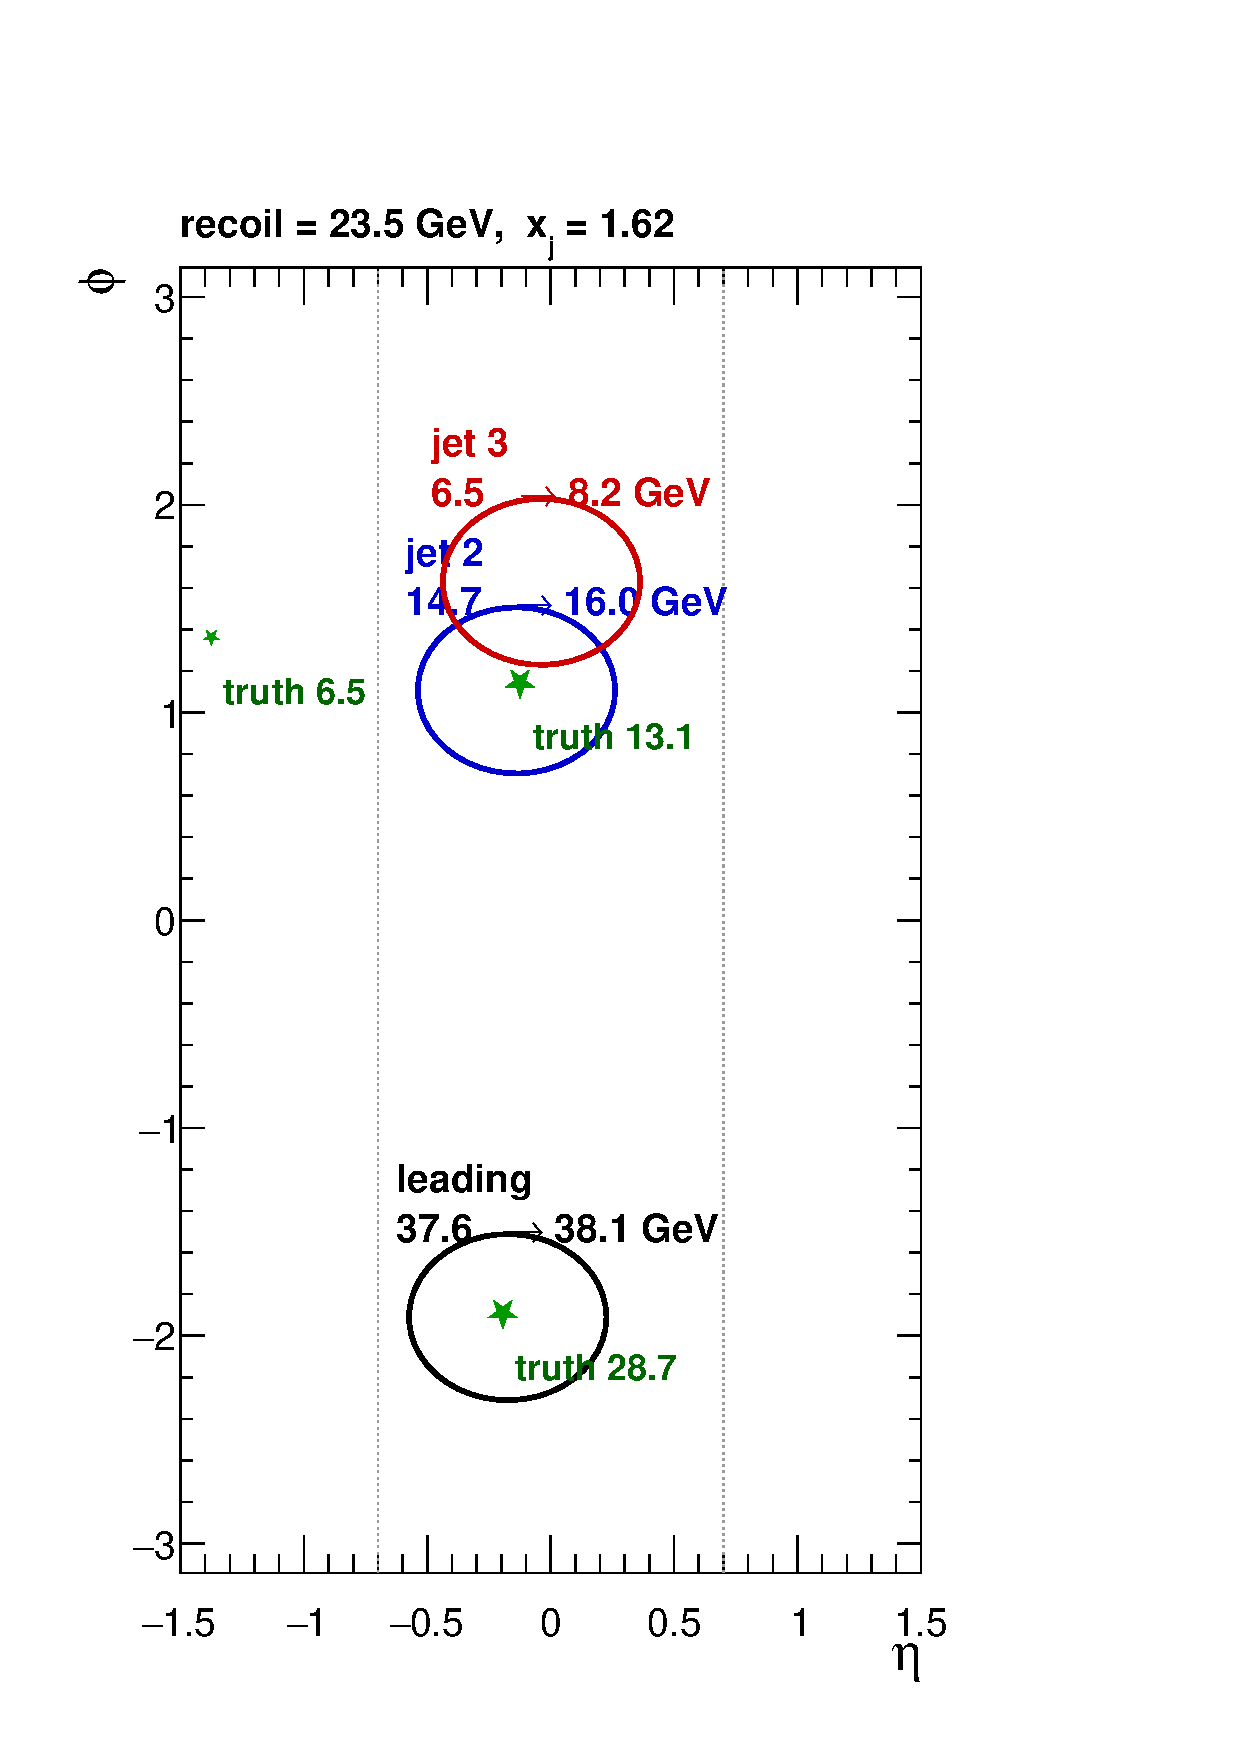
\includegraphics[height=0.83\textheight]{figs/event_display_3.pdf}
    \end{column}
    \begin{column}{0.29\textwidth}
      \centering
      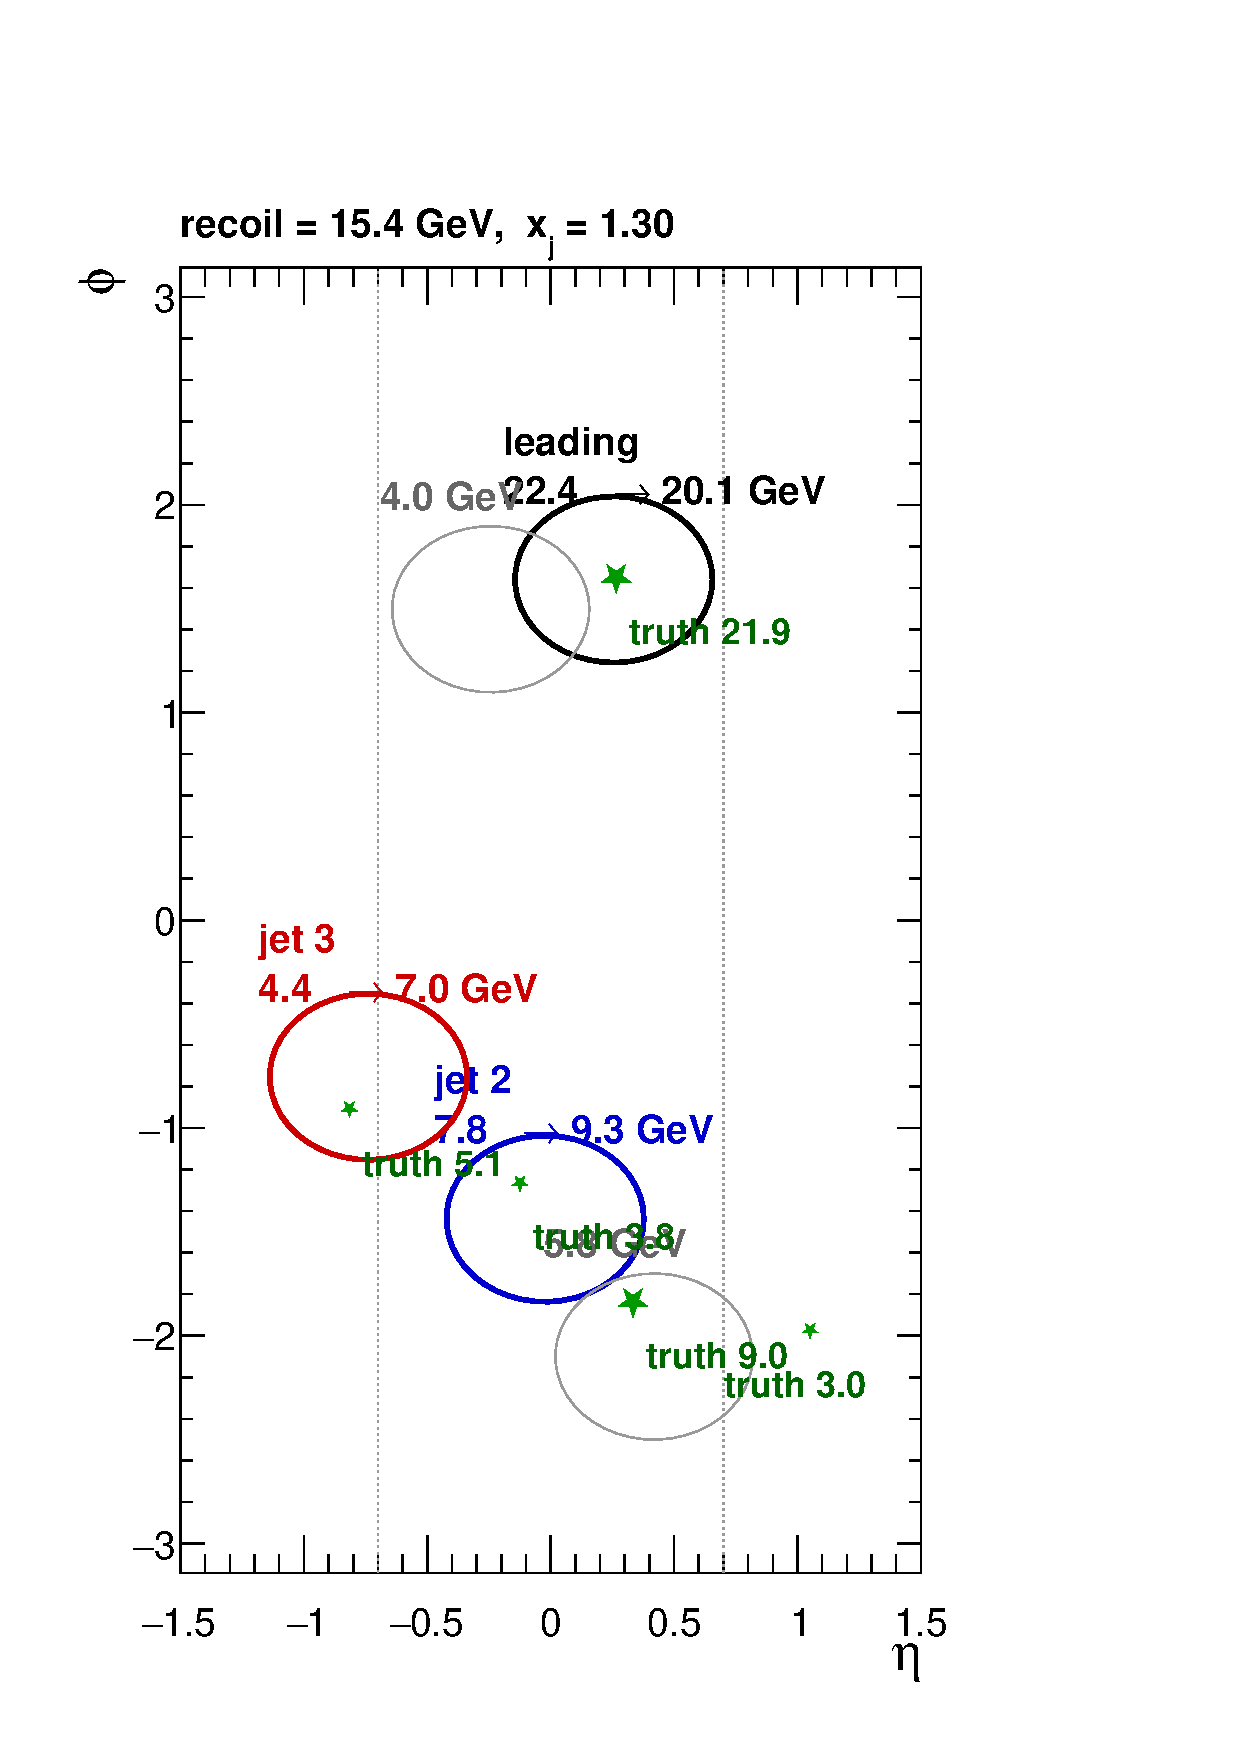
\includegraphics[height=0.83\textheight]{figs/event_display_5.pdf}
    \end{column}
    \begin{column}{0.38\textwidth}
      \small
      Pythia8 Jet20, R = 0.4: selected events with three reco jets but only two truth jets $\geq 7$ GeV.
      \vspace{0.4em}

      Reco jets show calibrated $\to$ smeared $p_T$; green stars are truth jets; dotted lines mark the acceptance.
      \vspace{0.4em}
      \begin{itemize}
        \item Left: jet 3 overlaps jet 2, so it is a split piece of the 13.1 GeV truth jet.
        \item Right: smearing pushes two soft jets over 7 GeV.
        \item The 9.0 GeV truth jet's reco partner (5.8 GeV) is not selected.
      \end{itemize}
    \end{column}
  \end{columns}
\end{frame}

% ------------------------------------------------------------------
\begin{frame}{How often this happens in the selected MC}
  \small
  Fraction of selected events with exactly two truth jets $\geq 7$ GeV
  (current selection, stitched Jet12/20/30).
  \vspace{0.5em}

  \centering
  \begin{tabular}{lcccc}
    \toprule
    R & Jet12 & Jet20 & Jet30 & cross-section weighted MC \\
    \midrule
    0.2 & 65.2\% & 73.2\% & 62.8\% & 68.3\% \\
    0.3 & 73.1\% & 72.3\% & 54.3\% & 72.3\% \\
    0.4 & 77.3\% & 68.7\% & 45.8\% & 73.3\% \\
    0.5 & 74.0\% & 54.1\% & 28.1\% & 72.1\% \\
    0.6 & 74.8\% & 52.8\% & 23.7\% & 73.7\% \\
    0.7 & 73.8\% & 46.5\% & 18.2\% & 73.3\% \\
    0.8 & 70.1\% & 50.5\% & 50.0\% & 70.0\% \\
    \bottomrule
  \end{tabular}
  \vspace{0.6em}
  \begin{itemize}
    \item About 70\% of the weighted MC sample, at every radius.
    \item The lower $\hat p_T$ samples, which dominate the low-$p_T$ bins, have the most.
    \item These are the events the new recoil smearing is applied to.
  \end{itemize}
\end{frame}

% ------------------------------------------------------------------
\begin{frame}{Proposed correction: smear the recoil, not the soft jets}
  \begin{itemize}
    \item Recoil $= |\vec p_{T,2} + \vec p_{T,3}|$.
    \item Current: smear jets 2 and 3 individually, then add them.
    \item Proposed, in events with exactly two truth jets $\geq 7$ GeV: add jets 2 and 3 unsmeared, then smear the sum once.
    \item The width comes from the same template, evaluated at the $p_T$ of the truth jet matched to the recoil.
    \item The recoil truth jet is the one not matched (in $\Delta R$) to the leading reco jet.
  \end{itemize}
  \vspace{0.5em}
  \small
  Jet20, R = 0.4, 20--25 GeV, two-truth-jet events, mean $\xj$:
  \vspace{0.3em}

  \centering
  \begin{tabular}{lccc}
    \toprule
    comparison & unsmeared & A: smear, then add & B: add, then smear \\
    \midrule
    same jets, cuts before smearing & 1.063 & 1.084 & 1.076 \\
    jets selected after smearing & 1.137 & 1.002 & 1.143 \\
    each cut on its own smeared recoil $\geq 15$ GeV & -- & 1.044 & 1.067 \\
    \bottomrule
  \end{tabular}
\end{frame}

% ------------------------------------------------------------------
\begin{frame}{Recoil spectra: smear-then-add vs add-then-smear}
  \begin{columns}[T]
    \begin{column}{0.49\textwidth}
      \centering
      \small Jets selected after smearing\\
      \includegraphics[width=\linewidth,page=5]{figs/recoil_smearsel.pdf}
    \end{column}
    \begin{column}{0.49\textwidth}
      \centering
      \small Each method cut on its own smeared recoil $\geq 15$ GeV\\
      \includegraphics[width=\linewidth,page=5]{figs/recoil_recoilcut.pdf}
    \end{column}
  \end{columns}
  \vspace{0.3em}
  \small
  \begin{itemize}
    \item Two individual smears at low-$p_T$ widths give a broader, harder recoil.
    \item Near a cut on a falling spectrum, that means more upward migration.
  \end{itemize}
\end{frame}

% ------------------------------------------------------------------
\begin{frame}{A recoil-only cut needs to stay inside both skims}
  \begin{itemize}
    \item Dropping the per-jet 7 GeV cuts gave data/MC $\approx 0.96$--$0.97$.
    \item Jet 3 below 7 GeV: 70\% of selected MC events, but only 34--40\% in data.
    \item The data skim requires three calib jets $\geq 7$ GeV; the MC skim accepts any flavor.
    \item So the event sample was defined by the two different skims.
  \end{itemize}
  \vspace{0.5em}
  \textbf{Adopted selection (option 1):}
  \begin{itemize}
    \item Leading $\geq 20$ GeV, jets 2 and 3 $\geq 7$ GeV each, recoil $\geq 14$ GeV.
    \item The 7 GeV cuts use each event's values before any recoil smearing.
    \item Two-truth-jet MC events use the recoil smearing; all others keep individual smearing.
  \end{itemize}
\end{frame}

% ------------------------------------------------------------------
\begin{frame}{Result: R = 0.2--0.5 within about 1\% below 35 GeV}
  \begin{columns}[T]
    \begin{column}{0.42\textwidth}
      \includegraphics[width=\linewidth,page=7]{figs/means_final.pdf}
    \end{column}
    \begin{column}{0.56\textwidth}
      \small
      R = 0.4, data/MC of $\langle\xj\rangle$:
      \vspace{0.3em}

      \begin{tabular}{lccccc}
        \toprule
        & 20--25 & 25--30 & 30--35 & 35--40 & 40--50 \\
        \midrule
        original & 1.077 & 1.067 & 1.063 & 1.037 & 1.034 \\
        reco smear & \good{1.012} & \good{1.001} & \good{0.990} & 0.983 & 0.961 \\
        truth smear & \good{1.007} & \good{0.997} & \good{0.993} & 0.983 & 0.958 \\
        \bottomrule
      \end{tabular}
      \vspace{0.5em}

      20--25 GeV bin, all radii (reco smear):
      \vspace{0.3em}

      \begin{tabular}{ccccccc}
        \toprule
        0.2 & 0.3 & 0.4 & 0.5 & 0.6 & 0.7 & 0.8 \\
        \midrule
        0.998 & 1.002 & 1.012 & 1.001 & 1.020 & 1.026 & 1.041 \\
        \bottomrule
      \end{tabular}
    \end{column}
  \end{columns}
\end{frame}

% ------------------------------------------------------------------
\begin{frame}{Result: $\xj$ distributions, R = 0.4}
  \centering
  \includegraphics[width=0.92\linewidth,page=7]{figs/dists_final.pdf}
  \small
  \begin{itemize}
    \item Data and MC shapes agree in every bin up to 40 GeV.
    \item The JER high/low variations bracket the nominal within about $\pm 0.5\%$.
  \end{itemize}
\end{frame}

% ------------------------------------------------------------------
\begin{frame}{Summary and next steps}
  \begin{itemize}
    \item The skim cut MC on calibrated $p_T$, while the analysis cut on smeared $p_T$; this is now fixed in the treemaker.
    \item Jet5 and Jet8 are removed, and Jet12 starts at truth $p_T = 0$.
    \item The large low-$p_T$ smearing width drove the remaining 2--3\% excess through soft jets crossing 7 GeV.
    \item Smearing the summed recoil in two-truth-jet events, with a 14 GeV recoil cut, brings R = 0.2--0.5 to within about 1\%.
  \end{itemize}
  \vspace{0.5em}
  \textbf{Open items}
  \begin{itemize}
    \item Provenance of the JER template: extra width or total data resolution?
    \item The same template feeds the $\gamma$+jet unfolding, so check its impact there.
    \item The ratio falls with leading $p_T$ (0.96 at 40--50 GeV, R = 0.4); watch it with more statistics.
    \item R $\geq 0.6$ is still 2--4\% high at low $p_T$, and its template is R = 0.4.
    \item Data trees: rerun with the finished reprocessing; herwig still to be regenerated.
  \end{itemize}
\end{frame}

\end{document}
